\chapter{Methodology}
\label{cha:methodology}

Using the information in Chapter~\ref{cha:background}, we will investigate each of the research questions by exhaustively generating all pairwise non-isomorphic graphs belonging to a specified graph class, potentially filter these graphs according to the relevant properties, and analyze the remaining graphs using algorithms developed as part of this thesis. In the case of RQ\ref{rq1}, this method could prove the existence of a 2-connected graph with circumference $11$ and empty $11$-cycle intersection, or establish the nonexistence of such a graph within the generated graph class(es). In the case of RQ\ref{rq2}, this could bring forth an example graph for a value $k$ where the graph is $2$-connected, planar, of minimum degree $4$, and has a $k$-cycle in every vertex-deleted subgraph and no larger cycle in the graph itself. Alternatively, this method could show no such graph exists within the generated class(es).

In this chapter, we explain in detail the computational framework used, what graph generators and tools were used, and the designed algorithms and the optimizations for each of the research questions, as well as the correctness tests performed to ensure the algorithms function as intended. We also explain a theoretical method used to find new results.

\section{Computational framework and package versions}

For RQ\ref{rq1}, we opted to generate 2-connected graphs, and to design and implement an algorithm that can check if a graph has circumference $k$, and compute the intersection of all $k$-cycles. For RQ\ref{rq2}, we generate 2-connected planar graphs with minimum degree 4, and we design and implement an algorithm that can check for what $k$ there exists a $k$-cycle in all vertex-deleted subgraphs of a graph, and if that graph has a cycle larger than $k$.

Since we will use multiple programs and processes to solve this problem, we use Linux's pipelining capabilities to efficiently pass output from one program as input to another. We use the \texttt{graph6} format, an \texttt{ASCII}-based encoding for graphs~\cite{article:jorik-jooken}, and all output and input of graphs are in this format. The output of the programs implemented in this thesis are in the \texttt{CSV} format, including a header. Each pipeline is implemented as a shell script, which connects the individual programs using Unix pipes, and records the total execution time from the start of graph generation until the completion of the analysis.

All algorithms are implemented using \texttt{C++}, and all implementations and packages are compiled using \texttt{g++} version \texttt{13.3.0}. The computations are run on a CPU model \texttt{Intel® Core™ Ultra 5 125U}, using the operating system \texttt{Linux Mint 22.3} with kernel \texttt{7.0.0-28-generic}. \texttt{Nauty} version \texttt{2.9.3} is used, and \texttt{plantri} version \texttt{5.5}.

\section{Generators used}

\subsection{Research Question \ref{rq1}: 2-connected, circumference 11, empty 11-cycles}[Research Question \ref{rq1}]

For the first research question, we use the generator \texttt{geng} from the \texttt{Nauty} package, since it is known to generate pairwise non-isomorphic graphs ``very quickly''~\cite{lib:nauty}, and can be set to generate specifically 2-connected graphs using the option \texttt{-C}. During the year, as seen in Table~\ref{tab:2con-nonhamil-2con}, we realized it was likely that most 2-connected graphs are Hamiltonian\
\footnote{The counts for the non-Hamiltonian 2-connected graphs are generated using the pipeline \texttt{./library/bin/generateUHG n H0} \texttt{|} \texttt{./library/bin/countg -c2}, which generates non-Ha\-mil\-to\-nian graphs, and then counts the number of graphs which are 2-connected}.
For that reason, we also utilized the generator \texttt{GenerateUHG}~\cite{lib:UHG}. This generator has the option \texttt{H<x>} where \texttt{<x>} is the number of unique Hamilton cycles in the generated graphs. By setting this number to 0, we can generate specifically non-Hamiltonian graphs. \texttt{GenerateUHG} does not support an option for generating (2-)connected graphs, which is why we opted to extend the pipeline by using \texttt{pickg} from the \texttt{Nauty} package~\cite{lib:nauty} using the option \texttt{-c2} to select only the 2-connected graphs generated. This means that more graphs would be generated by \texttt{GenerateUHG}, but only those that are potentially interesting would be sent to the self-designed program. We suspected \texttt{pickg} to be significantly faster than the self-designed program as seen in Section~\ref{sec:1-timing}, so this program was not going to be a bottleneck of the pipeline. Table~\ref{tab:2con-nonhamil} shows that the total number of graphs generated for 13 nodes (and possibly higher) is still lower using this second method of generating non-Hamiltonian graphs, than if all 2-connected graphs of order 13 were generated instead.

The total number of 2-connected graphs of order 13 or higher, whether non-Hamiltonian or not, still proved to be too large a number to feasibly generate and check all graphs of that class, as seen in Section~\ref{sec:1-timing}. Both \texttt{geng} and \texttt{GenerateUHG} have options to reduce the generated graphs by setting an upper bound of the maximum degree of the generated graphs. For \texttt{geng}, this is the option \texttt{-D<x>}, while for \texttt{GenerateUHG} this is simply \texttt{D<x>}, where \texttt{<x>} is this upper bound. To make generation feasible, the following generation schema was used with respect to the maximum degree. We generate all graphs with maximum degree at most 3 of order 13, increasing the order by 1 if computation was still done in a reasonable time. Based on these timings, we similarly increased the upper bound on the maximum degree.

One reasoning for using this schema is that $G_{4,2}$, $G_{5,2}$, and $G_{6,2}$ from Section~\ref{sec:tube-graph}, which are solutions to the question by van Aardt et al.\ for circumference $k \in \{10, 13, 16\}$ respectively, all have maximum degree 3, and an order equal to their circumference $+ 2$. Perhaps a solution for circumference $11$, should it exist, is similar to these graphs, perhaps with some additional edges and/or vertices.

Lastly, an attempt using \texttt{plantri}~\cite{lib:plantri} was also used. Since $G_{5,2}$ is planar, and the number of planar 2-connected graphs is much smaller, as seen in Table\ref{tab:2con-planar}, we also generate all planar graphs of order 13 which are 2-connected. The generator \texttt{plantri} supports the options \texttt{-p} to generate general planar graphs (rather than the default of triangulations~\cite{lib:plantri}), \texttt{-c2} to generate 2-connected planar graphs (this also sets the minimum degree to at least 2, from the default of 3), and \texttt{-g} to force the output to be in the \texttt{graph6} format. As mentioned in Section~\ref{sec:generators}, there may be some isomorphic 2-connected graphs as the graphs are only pairwise non-isomorphic with respect to the embedding on a sphere.

Thus, the resulting generation pipelines are as follows.
\begin{verbatim}
generateUHG <n> H0 D<d> | pickg -c2
geng -CD<d> <n>
plantri <n> -gpc2
\end{verbatim}
Here, \texttt{<n>} stands for the order, and \texttt{<d>} stands for the upper bound of the maximum degree of the graphs generated.

\begin{table}
  \centering
  \caption{Amount of 2-connected graphs~\cite{data:integer-sequence} and 2-connected non-Hamiltonian graphs~\cite{lib:UHG} per order of the graph $n$}
  \label{tab:2con-nonhamil-2con}
  \begin{tabular}{rrr}
    \hline\\
    $n$ & 2-connected & Non-Hamiltonian 2-connected \\
    \hline \\
    1 & 0 & 0 \\
    2 & 1 & 0 \\
    3 & 1 & 0 \\
    4 & 3 & 0 \\
    5 & 10 & 2 \\
    6 & 56 & 8 \\
    7 & 468 & 85 \\
    8	& 7\,123 & 927 \\
    9	& 194\,066 & 16\,983 \\
    10 & 9\,743\,542 & 438\,424 \\
    11 & 900\,969\,091 & 17\,813\,067 \\
    \hline
  \end{tabular}
\end{table}

\begin{table}
  \centering
  \caption{Amount of 2-connected graphs~\cite{data:integer-sequence} and of non-Hamiltonian graphs~\cite{lib:UHG} per order of the graph $n$}
  \label{tab:2con-nonhamil}
  \begin{tabular}{rrr}
    \hline\\
    $n$ & 2-connected & Non-Hamiltonian \\
    \hline \\
    1 & 0 & 1 \\
    2 & 1 & 2 \\
    3 & 1 & 3 \\
    4 & 3 & 8 \\
    5 & 10 & 26 \\
    6 & 56 & 108 \\
    7 & 468 & 661 \\
    8	& 7\,123 & 6\,150 \\
    9	& 194\,066 & 97\,585 \\
    10 & 9\,743\,542 & 270\,050 \\
    11 & 900\,969\,091 & 135\,841\,840 \\
    12 & 153\,620\,333\,545 & 12\,568\,984\,762 \\
    13 & 48\,432\,939\,150\,704 & 2\,179\,513\,027\,405 \\
    \hline
  \end{tabular}
\end{table}

\begin{table}
  \centering
  \caption{Amount of 2-connected graphs~\cite{data:integer-sequence} and planar 2-connected graphs~\cite{data:planar-2con-count} per order of the graph $n$}
  \label{tab:2con-planar}
  \begin{tabular}{rrr}
    \hline\\
    $n$ & 2-connected & Planar 2-connected \\
    \hline \\
    1 & 0 & 0 \\
    2 & 1 & 0 \\
    3 & 1 & 1 \\
    4 & 3 & 3 \\
    5 & 10 & 9 \\
    6 & 56 & 44 \\
    7 & 468 & 294 \\
    8	& 7\,123 & 2\,893 \\
    9	& 194\,066 & 36\,496 \\
    10 & 9\,743\,542 & 545\,808 \\
    11 & 900\,969\,091 & 9\,029\,737 \\
    12 & 153\,620\,333\,545 & 159\,563\,559 \\
    13 & 48\,432\,939\,150\,704 & 2\,952\,794\,985 \\
    \hline
  \end{tabular}
\end{table}


\subsection{Research Question \ref{rq2}: on planar 2-connected graphs with minimum degree 4}[Research Question \ref{rq2}]

\begin{samepage}
For clarity, we repeat the second research question here. ``For which values of $k$ is it true that if in a planar graph $G$ with minimum degree at least $4$ all vertex-deleted subgraphs contain a cycle of length $k$, then $G$ contains a cycle of length greater than $k$?''
\end{samepage}

For this research question, only 2-connected planar graphs with minimum degree of at least 4 are relevant. Both \texttt{GenerateUHG} and \texttt{plantri} allow generating planar graphs, but only \texttt{plantri} has options to generate 2-connected planar graphs with minimum degree at least 4. Again, this generator only generates non-isomorphic 2-connected graphs where isomorphism is defined with reference to the embedding on a sphere. Despite this redundancy, we suspect that generating 2-connected planar graphs with minimum degree at least 4 using \texttt{plantri} remains more efficient than generating planar non-Hamiltonian graphs and checking for 2-connectedness and minimum degree. Additionally, because of Observation~\ref{obs:3con-hamiltonian}, we know that all 3-connected planar graphs with less than 23 vertices and with minimum degree at least 4 must be Hamiltonian. Since the aim of this thesis on this research question is to find negative examples of RQ\ref{rq2}, i.e. graphs $G$ with a value $k$ for which the statement in the research question is \textit{not} true, we can limit our search to specifically the graphs with \textit{connectivity} 2, i.e. 2-connected but not 3-connected, as seen in Table~\ref{tab:2con-planar-m4}. The \texttt{plantri} generator also has an option for this. This brings us to the following pipeline.
\begin{verbatim}
plantri <n> -gpm4c2x
\end{verbatim}
Here, \texttt{-g} is for outputting in the \texttt{graph6} format, \texttt{-p} for generating general planar graphs, \texttt{-m4} for generating graphs with minimum degree at least 4, and \texttt{-c2x} for generating graphs with connectivity exactly 2. Lastly, \texttt{<n>} stands for the order of the graphs generated. Using Observation~\ref{obs:2con-n14}, the graphs which could potentially be negative examples should have at least order 14. By Observation~\ref{obs:3con-hamiltonian} from before, using this pipeline could make definitive statements on values $k$ for graphs up to (and including) order 22.

\begin{table}
  \centering
  \caption{Amount of generated 2-connected planar graphs with (parameters \texttt{pgm4c2}), and generated planar graphs with connectivity 2 (with parameters \texttt{pgm4c2x}) per order of the graph $n$}
  \label{tab:2con-planar-m4}
  \begin{tabular}{rrr}
    \hline\\
    $n$ & 2-connected & Connectivity 2 \\
    \hline \\
    6 & 1 & 0 \\
    7 & 1 & 0 \\
    8	& 4 & 0 \\
    9	& 14 & 0 \\
    10 & 69 & 2 \\
    11 & 445 & 17 \\
    12 & 3\,754 & 239 \\
    13 & 34\,563 & 2\,800 \\
    14 & 341\,758 & 34\,215 \\
    15 & 3\,470\,706 & 406\,005 \\
    16 & 35\,958\,178 & 4\,759\,110 \\
    17 & 377\,489\,455 & 55\,224\,800 \\
    \hline
  \end{tabular}
\end{table}

\subsubsection{List of graphs}

As mentioned in Section~\ref{sec:generators}, we were also given access to a list of non-Hamiltonian, 2-connected planar graphs with minimum degree 4 for orders ranging from 14 up to and including 20. In Section~\ref{sec:2-timing}, we will see that the former generation becomes infeasible to perform at roughly order 18. Therefore, this list of graphs extends the class of graphs for which we can make definitive statements to those of order up to 20. These lists consist of a file per order of the graphs, containing a \texttt{graph6} string (and thus graph) per line, similar to the output of all generators discussed so far. Therefore, we can use the Unix \texttt{<} operator to pipe this data directly into our own program. 

\section{Algorithms designed}
\label{sec:algorithms}
% Finding the Intersection of longest k-cycles

In the previous section, we've shown we generate 2-connected graphs, with potentially some additional interesting properties, for the pipeline of RQ\ref{rq1}. This leaves us with the problem of creating a program which can check whether the generated graphs have no vertex in all 11-cycles, and if the graph has circumference 11. For RQ\ref{rq2}, we generate 2-connected planar graphs with minimum degree 4, and thus the program for that pipeline must identify graphs which have $k$-cycles in all vertex-deleted subgraphs, and no longer cycle in the graph itself. We will first create an algorithm for RQ\ref{rq1}, then show that the problem for RQ\ref{rq2} can be reduced to a problem that is almost identical to that of RQ\ref{rq1}.

\subsection{Circumference $k$ with intersection of $k$-cycles}

We generalize the problem for RQ\ref{rq1} to checking if a graph has circumference $k$, and has no vertex meeting every $k$-cycle for any given $k$. Doing so allows us to test the final program on the known graphs $G_{p,\ell}$. Finding the longest cycle in a general graph, known as longest cycle problem, ``is well known as NP-complete.''~\cite{article:longest-cycle-np}, meaning there is no known polynomial algorithm for solving it and remains computationally expensive. The approach to solving this problem in this thesis is to enumerate all cycles, which lets us determine if a cycle of length $k$ exists and/or a cycle longer than $k$. This enumeration also provides an easy method for computing the required $k$-cycle intersection, as we just take the intersection of all found $k$-cycles. Thus, we need an algorithm for enumerating all cycles efficiently in a graph.

\subsubsection{Enumeration of all cycles}

The approach used in this thesis to enumerate all cycles of a graph $G$ is a depth-first search over the vertices. The algorithm starts from each vertex $v_{\text{start}} \in V(G)$ in turn. For each starting vertex, $v_{\text{start}}$ is added to the current path $P=[v_{\text{start}}]$, and a set of its unvisited neighbors $A(v_{\text{start}})$ is initialized. The following steps are then repeated until $P$ is empty.

First, if the last vertex $v_{\text{last}}$ in $P$ has no unvisited neighbors, i.e., $A(v_{\text{last}})=\emptyset$, then $v_{\text{last}}$ is removed from $P$. Otherwise, an unvisited neighbor $v_{\text{next}} \in A(v_{\text{last}})$ is selected as the next candidate vertex. This candidate may be the starting vertex $v_{\text{start}}$.

If $v_{\text{next}}=v_{\text{start}}$ and $P$ contains at least three vertices, a cycle has been found. The vertices in $P$ are the vertices of the cycle, whose length is the length of $P$. If $v_{\text{next}} \neq v_{\text{start}}$, then $v_{\text{next}}$ is appended to $P$, and its list of unvisited neighbors is initialized as
\[
A(v_{\text{next}}) =
(N(v_{\text{next}}) \setminus V(P)) \cup \{v_{\text{start}}\}
\]
where $N(v_{\text{next}})$ is the set of neighbors of $v_{\text{next}}$. The search then continues from $v_{\text{next}}$.

The algorithm described above is not yet efficient, as each cycle is enumerated twice for every vertex it contains. This is because every vertex of the cycle is considered as a possible starting vertex, and, for each starting vertex, the cycle is discovered in both possible traversal directions. Thus, a cycle of length $k$ is enumerated $2k$ times. We can reduce the number of enumerations by exploiting a property of the way vertices are represented in the source code of this thesis. Vertices are represented by integers from $0$ to $n-1$, where $n$ is the order of the graph. Consequently, the vertices have an ordering.

This ordering allows us to require that the starting vertex of a cycle is its minimum vertex. During the search, a new vertex is only considered as a candidate if it is larger than the starting vertex. This ensures that every cycle is only considered from its minimum vertex, reducing the number of enumerations from $2k$ to $2$ for a cycle of length $k$.

Additionally, the vertex ordering can be used to restrict the search to only one of the two possible directions. We do this by requiring there must be a fixed order between first and last vertex of the cycle, excluding the starting vertex. For example, if the first vertex is required to be smaller in order than the last vertex, cycles encountered in the opposite direction are ignored. This reduces the number of enumerations from two to one, meaning that every cycle is enumerated exactly once.

\subsubsection{Halting cycle enumeration early}

This algorithm allows us to enumerate all cycles of the graph exactly once. From this enumeration, we can determine if the circumference of a graph is equal to some value $k$, larger than $k$, or smaller than $k$. If during enumeration, we find a cycle that is larger than $k$, we know the circumference to be larger than $k$, and can halt cycle enumeration early. If the enumeration completed and no $k$-cycle is found, we know that the graph must have circumference less than $k$. If, instead, a $k$-cycle is found, then the circumference is equal to $k$.

Additionally, we can also stop enumeration early if during enumeration we know that no remaining cycle found has length $k$ or larger. This can be done by reducing the allowed starting vertices to those that still allow at least $k$ vertices. By starting from the lowest ordered vertex as the starting vertex, choosing the next lowest ordered vertex every iteration, we can halt enumeration early when the remaining starting vertices, which are the minimum vertices of the cycles, allow for only $k-1$ vertices as part of any new cycle.

\subsubsection{Computing the $k$-cycle intersection}

During enumeration, we must also compute the intersection of all $k$-cycles. Set the initial intersection $I$ equal to all vertices of the graph $V(G)$ at the start of enumeration. Whenever a $k$-cycle $C$ is found, set $I$ equal to the intersection of the current intersection and the vertices of the $k$-cycle $I_{\text{new}} = I \cap V(C)$. The result at the end of the enumeration will be the intersection of all $k$-cycles if there are any, or all vertices otherwise. If there are no $k$-cycles, then the computed intersection will remain all vertices of the graph $V(G)$.

% --- COMMENT: KEEP IN METHODOLOGY. ---

\begin{algorithm}
\caption{\textsc{FindIntersectionK}$(G,k,\prec)$}
\label{alg:find-k-intersection}

\begin{algorithmic}[1]
\Require Graph $G$, integer $|V(G)|>k>2$, and a total ordering on $V$
\Ensure intersection of all $k$-cycles $\textit{intersection}$ and circumference $c(G)=k$

\State $\textit{intersection} \gets V(G)$
\ForAll{$s \in V(G)$ ascending}
\State $\textit{path} \gets [s]$
\While{$\textit{path}$ is not empty}
    \State $u \gets$ the last vertex in $\textit{path}$
    \If{no unvisited neighbor of $u$}
        \State remove $u$ from $\textit{path}$
        \Comment Including its visited neighbors
        \State \textbf{continue}
    \EndIf
    \State {$v \gets$ an unvisited vertex, and unvisited neighbor of $u$}
    \State mark $v$ as visited neighbor of $u$
    \If{$v=s$}
        \State $\ell \gets |\textit{path}|$
        \If{$\ell > k$}
            \State \Return $\text{LARGER\_THAN\_K}$
        \EndIf
        \If{$\ell = k$}
            \State $\textit{intersection} \gets
            \textit{intersection} \cap \textit{path}$
        \EndIf
        \State \textbf{continue}
    \EndIf
    \If{$s \prec v$}
        \State add $v$ to $\textit{path}$
    \EndIf
\EndWhile
\EndFor

\If{$\textit{intersection} = V(G)$}
    \State \Return $\text{SMALLER\_THAN\_K}$
\EndIf
\State \Return $\text{EQUAL\_TO\_K}$
\end{algorithmic}
\end{algorithm}

% --- COMMENT: KEEP IN METHODOLOGY. This is the central algorithm and should remain here. ---

\section{Checking vertex-deleted subgraphs for k-cycles}

% --- COMMENT: KEEP IN METHODOLOGY. ---

\todo{Add RQ2 again for clarity}

% --- COMMENT: KEEP IN METHODOLOGY. ---

This section introduces the algorithm for RQ\ref{rq2}. The approach is similar to RQ\ref{rq1}: we generate planar graphs with minimum degree 4, and check for each graph if in every vertex-deleted subgraph there exists a $k$-cycle, that there then is a cycle larger than $k$. Trivially, if a vertex-deleted subgraph of a graph $G$ has a $k$-cycle, then the graph $G$ itself also has a $k$-cycle. As a result, for a graph $G$ can only be a negative example of RQ\ref{rq2}, there must be a $k$-cycle in every vertex-deleted subgraph of $G$ and $G$ must also have circumference $k$. From this, we decided to focus our algorithm on finding negative examples, as we can assume all other graphs to be positive examples.
% --- COMMENT: KEEP IN METHODOLOGY. This explains the computational strategy for RQ2. However, the definitions of vertex-deleted subgraphs, circumference, and relevant graph properties should be available in Background. ---

\begin{theorem}
  \label{theorem:intersection-vertex-deletion}
  A graph $G$ has a $k$-cycle in every vertex-deleted subgraph, and no cycle larger than $k$ in $g$ if and only if the intersection of the vertices of all $k$-cycles in the graph is empty, and $G$ has circumference $k$.
\end{theorem}

\begin{proof}
  Assume $G$ has a $k$-cycle in every vertex-deleted subgraph, and no cycle larger than $k$ exists in $G$. $G$ must have at least one $k$-cycle, denoted $C$, and therefore must have circumference $k$. The intersection of all $k$-cycles must be at most the vertices $V(C) \subset V(G)$. Per the assumption, for every vertex $v_i \in V(G)$ there must be a $k$-cycle $C_i'$ in $G$ avoiding the vertex $v_i$, including those vertices $v_i \in V(C)$. As a result, the intersection of all $k$-cycles is at most
  $$
  \bigcap_{i} C_i' \cap C = \emptyset
  $$
  and thus the intersection of all $k$-cycles must be empty.

  Now assume $G$ has circumference $k$ and the intersection of all $k$-cycles is empty. $G$ cannot be hamiltonian, as otherwise the intersection of the vertices of all $k$-cycles must be the vertices $V(G)$. $G$ must have at least one $k$-cycle $C$, which avoids all vertices $v_{\text{out}} \in V(G) \setminus V(C)$. Additionally, since the intersection of all $k$-cycles is empty, there must be a $k$-cycle for every vertex $v_{\text{in}} \in V(C)$ which avoids $v_{\text{in}}$. As a result, there exists a $k$-cycle avoiding every vertex $v \in V(C) \cup (V(G) \setminus V(C)) = V(G)$, and therefore every vertex-deleted subgraph of $G$ has a $k$-cycle.

  We conclude that for a graph $G$, $G$ has a $k$-cycle in every vertex-deleted subgraph and has circumference $k$ if and only if the intersection of the vertices of all $k$-cycles in the graph is empty.
\end{proof}

% --- COMMENT: KEEP IN METHODOLOGY if this theorem is specifically the mathematical justification for the implemented algorithm. However, if the Literature Study chapter is intended to contain the theoretical development behind the research questions, the theorem could be moved to Background/Theory and Methodology could simply state that the algorithm exploits this equivalence. My preference: keep it here if you proved it yourself and use it directly to justify the implementation. ---

This result allows us to reuse most of Algorithm~\ref{alg:find-k-intersection}. To adapt it to RQ\ref{rq2}, instead of keeping track of the intersection of all $k$-cycles for an arbitrary value $k$, we must keep track of the intersection of the longest currently found cycles of the graph. This means that during execution, if a longer cycle is found than the current length of the longest cycles found, instead of halting early, we simply set the intersection of the longest cycles to the vertices of that new cycle.

% --- COMMENT: KEEP IN METHODOLOGY. This describes the adaptation of the algorithm for RQ2. ---

Thomassen has shown~\cite{article:thomassen} that for every planar graph with minimum degree 4 of order $n$, if the graph has an $(n-1)$-cycle in every vertex-deleted subgraph, it must also be hamiltonian. This mean we can still halt the algorithm early, namely when a cycle is found of length $n-1$ or $n$.

% --- COMMENT: The cited theorem itself belongs naturally in Background/Literature Study as prior theoretical work. The methodological consequence ("we can still halt the algorithm early") belongs here. Consider citing the theorem in Background and briefly invoking it here. ---

\subsection{Studying the Gadget}
\label{sec:gadget}

% --- COMMENT: This subsection should probably MOVE to Background/Literature Study if it primarily explains the known construction and its structural properties. If the "studying the gadget" work is genuinely a research method developed in this thesis, retain a shortened version in Methodology describing the procedure you used to investigate the gadget. The results/insights discovered from this study should then be presented in Results/Analysis rather than Methodology. ---

The construction by C. T. Zamfirescu starts off from two identical cycles with respective vertices connected. This graph is then modified, resulting in graphs with the desired properties. Studying this base graph, which we call a gadget, and seeing what properties it has and how modifying it results in the desired graphs could lead to new insights as to how to modify it differently to find new results for RQ\ref{rq2}.

% --- COMMENT: Likely Background/Literature Study if this is explaining the known construction. If it describes your research strategy, keep only the methodological part ("we study the base graph and modifications") in Methodology. ---

In this thesis, we look deeper into the types of cycles that can be created from this gadget, and how inserting vertices on their edges changes the length of these cycles. It is this approach that has led to new negative results to the question of RQ\ref{rq2}.

% --- COMMENT: The description of the approach can remain in Methodology, but the claim that it "has led to new negative results" is a result/conclusion and should probably be moved to the Results chapter. ---

\todo{Correctness tests, including tests on House of Graphs database}

\section{Conclusion}
\todo{Conclusion}
The final section of the chapter gives an overview of the important results
of this chapter. This implies that the introductory chapter and the
concluding chapter don't need a conclusion.

% --- COMMENT: KEEP/REWORK IN METHODOLOGY. This is a chapter conclusion, although the current text is placeholder/template text and does not actually summarize this chapter. It should eventually summarize the methodology: selected graph generators and parameters, computational pipelines, algorithms, and validation/testing. ---

\begin{figure}
  \centering
  \label{fig:pipeline-1}
  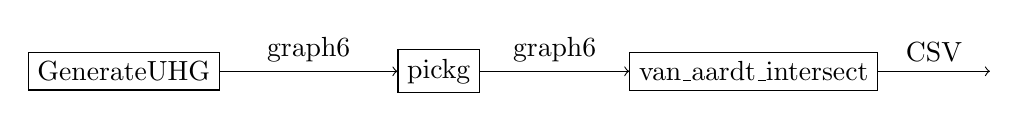
\begin{tikzpicture}[node distance=4cm, auto]
  \node[draw, rectangle] (gen) {GenerateUHG};
  \node[draw, rectangle, right of=gen] (filter) {pickg};
  \node[draw, rectangle, right of=filter] (analysis) {van\_aardt\_intersect};

  \draw[->] (gen) -- node {graph6} (filter);
  \draw[->] (filter) -- node {graph6} (analysis);
  \draw[->] (analysis) -- node {CSV} ++(3,0);
  \end{tikzpicture}
  \caption{The pipeline for RQ\ref{rq1}}
\end{figure}

% --- COMMENT: KEEP IN METHODOLOGY. This is an actual description of the computational pipeline. It should probably be introduced in General Structure and/or referenced from the generator-selection subsection. ---

\begin{figure}
  \centering
  \label{fig:pipeline-2}
  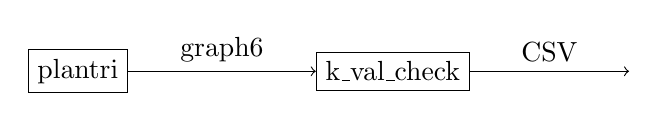
\begin{tikzpicture}[node distance=4cm, auto]
  \node[draw, rectangle] (gen) {plantri};
  \node[draw, rectangle, right of=gen] (analysis) {k\_val\_check};

  \draw[->] (gen) -- node {graph6} (analysis);
  \draw[->] (analysis) -- node {CSV} ++(3,0);
  \end{tikzpicture}
  \caption{The pipeline for RQ\ref{rq2}}
\end{figure}

% --- COMMENT: KEEP IN METHODOLOGY. This is an actual computational pipeline. ---

% --- COMMENT: OVERALL STRUCTURAL RECOMMENDATION:
% The Background/Literature Study chapter should probably absorb:
%   1. General definition and purpose of graph generators.
%   2. Overview of relevant generator packages and the graph classes they generate.
%   3. General discussion of graph isomorphism and graph6, if needed.
%   4. Definitions/properties of all relevant graph classes: connected, 2-connected, 3-connected, planar, minimum degree, Hamiltonian, non-Hamiltonian, hypohamiltonian, circumference, etc.
%   5. The prior result about 3-connected planar graphs of minimum degree 4 up to 22 vertices.
%   6. Prior work and known graph lists from Goedgebeur.
%   7. Zamfirescu's construction and its figures.
%   8. The gadget and known constructions derived from it, insofar as they are prior/theoretical background.
%   9. The modified Petersen construction and its significance for RQ1.
%  The Methodology chapter should then contain:
%   1. General computational pipeline.
%   2. Which generators were selected for each RQ and why.
%   3. Exact generator parameters and filtering steps.
%   4. How existing graph lists were incorporated into the search.
%   5. The cycle-intersection algorithm.
%   6. The RQ2 algorithm and its adaptation from RQ1.
%   7. Algorithmic optimizations and data structures.
%   8. Implementation language and implementation choices.
%   9. Correctness tests and validation.
%  This would align well with the intended Background TODO:
%     \todo{Add all theoretical background here from other chapters}
%     \section{Generators}
%     \todo{maybe a section about the different generators that exist, citing JJ}
%     \section{Graphs}
%     \todo{maybe a section on all relevant graphs to this paper}
%  In particular, the Background chapter can establish the "menu" of available generators and the relevant graph-theoretic concepts, while Methodology says: "Given this landscape, we selected X for RQ1 and Y for RQ2, configured them as follows, and connected them to our algorithms in these pipelines." This avoids duplicating the same explanations in both chapters.
